% !TeX program = lualatex
\documentclass[12pt, a4paper]{article}
\usepackage{fullpage}
\usepackage{subfiles}
\usepackage{fontspec}
\usepackage{libertine}
\usepackage{xcolor}
\usepackage{GotIn}
\usepackage{geometry}
\usepackage{multicol}
\usepackage{multicolrule}
\usepackage{graphicx}
\usepackage{enumitem}
\usepackage[autocompile]{gregoriotex}
\usepackage[latin,french]{babel}


\geometry{top=2cm, bottom=2cm}
% \pagestyle{empty}

\definecolor{red}{HTML}{C70039}
% \input GoudyIn.fd
% \newcommand*\initfamily{\usefont{U}{GoudyIn}{xl}{n}}

\input Acorn.fd
\newcommand*\initfamily{\usefont{U}{Acorn}{xl}{n}}
% cette ligne ajoute de l'espace entre les portées
% \grechangedim{baselineskip}{60pt}{scalable}

\begin{document}
  \gresetlinecolor{gregoriocolor}

  \begin{center}
    \textcolor{red}{\large{Salut du Très Saint Sacrement}}\\
    \textit{Chant d'exposition}
  \end{center}

  \smallskip
  \begin{figure}[h!]
    \centering
    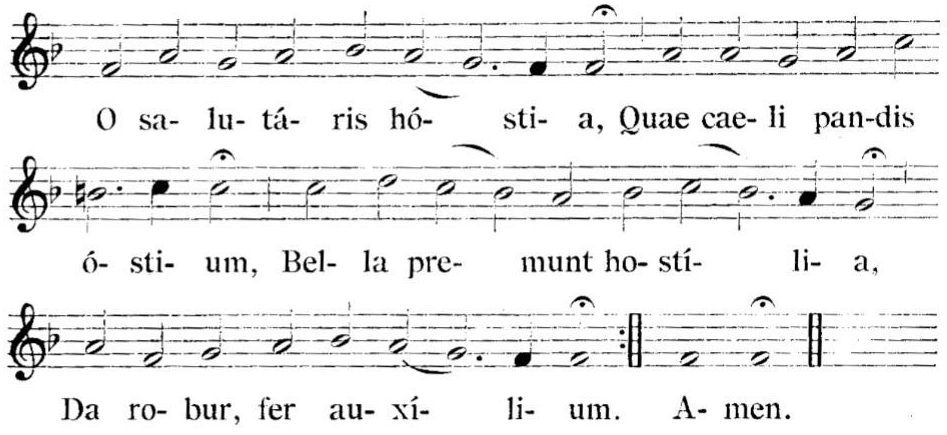
\includegraphics[width=\linewidth]{../ordinaires/o-salutaris.jpg}
  \end{figure}

  \begin{center}
    \begin{footnotesize}
      \textit{
        Ô réconfortante
        Hostie, Qui nous
        ouvres les portes du
        ciel, les armées ennemies
        nous poursuivent,
        Donne-nous la force,
        porte-nous secours.
      }
    \end{footnotesize}
  \end{center}

  \begin{multicols}{2}
    \begin{flushright}
      Uni trinoque Domino\\
      Sit sempiterna gloria :\\
      Qui vitam sine termino,\\
      Nobis donet in patria. Amen.\\
    \end{flushright}
    \columnbreak
    \textit{
      Au Seigneur unique en trois personnes,\\
      La gloire éternelle;\\
      qu'il nous donne en son Royaume\\
      La vie qui n'aura pas de fin. Amen\\
    }
  \end{multicols}
  \bigskip
  \begin{center}
    \rule{2cm}{0.4pt}
  \end{center}

  \newpage

  % \begin{center}
  %   \textcolor{red}{\normalsize{Antienne à la Sainte Vierge.}}\\
  % \end{center}
  \begin{center}
    \textcolor{red}{\large{Salve Regína}}\\
    \begin{footnotesize}
      \textit{
      Du Dimanche de Pâques jusqu'au Vendredi après la Pentecôte inclusivement.
      }
    \end{footnotesize}
  \end{center}

  \gresetinitiallines{1}
  \greillumination{\initfamily\fontsize{11mm}{11mm}\selectfont S}
  \gregorioscore{an--salve_regina--solesmes}
  \medskip
  \begin{footnotesize}
    \textit{
      Salut, ô Reine, Mère de Miséricorde, notre vie, notre douceur, et notre espérance, salut. Vers vous nous élevons nos cris, pauvres exilés, malheureux enfants d'Eve. Vers vous nous soupirons, gémissant et pleurant dans cette vallée de larmes. De grâce donc, ô notre Avocate, tournez vers nous vos regards miséricordieux. Et, après cet exil, montrez-nous Jésus, le fruit béni de vos entrailles. Ô clémente, ô miséricordieuse, ô douce Vierge Marie.  
    }
  \end{footnotesize}

  \begin{multicols}{2}
    \parindent=0pt
    \begin{flushright}
      \textcolor{red}{\Vbar.} Ora pro nobis, Sancta Dei Génitrix.\\
      \textcolor{red}{\Rbar.} Ut digni efficiamur promissionibus Christi.\\
    \end{flushright}

    \columnbreak
    
    \textit{\textcolor{red}{\Vbar.} Priez pour nous, Sainte Mère de Dieu. \\
    \textcolor{red}{\Rbar.} Afin que nous soyons rendus dignes des promesses du Christ.}\\
  \end{multicols}

  \begin{multicols}{2}
    \parindent=0pt
    Omnípotens sempitérne Deus, qui gloriósæ Vírginis Matris Maríæ corpus et ánimam, ut dignum Fílii tui habitáculum effici mererétur, Spíritu Sancto cooperánte, præparásti : \textcolor{red}{†} da, ut, cujus commemoratióne lætámur, \textcolor{red}{*} ejus pia intercessióne, ab instántibus malis et a morte perpétua líberémur.\\ Per eúmdem Christum Dóminum nostrum.\\ 
    \textcolor{red}{\Rbar.} Amen.

    \columnbreak

    \textit{Dieu tout-puissant et éternel, qui avez préparé le corps et l’âme de la glorieuse Vierge et Mère Marie afin d’en faire une demeure digne de votre Fils, avec le concours du Saint-Esprit ; faites que, par la prière maternelle de celle dont nous évoquons avec joie la mémoire, nous soyons affranchis du mal présent et de la mort éternelle.\\
    Amen.
    }
  \end{multicols}


  \newpage

  \begin{center}
    \textcolor{red}{\large{En l'honneur Du Saint Sacrement}}
  \end{center}

  \gresetinitiallines{1}
  \greillumination{\initfamily\fontsize{11mm}{11mm}\selectfont T}
  \gregorioscore{../ordinaires/hy--tantum_ergo--solesmes}

  \begin{center}
    \begin{footnotesize}
      \begin{enumerate}[label=\textcolor{red}{\emph{\arabic*}}]
        \item \textit{Devant un sacrement si grand, prosternons-nous, adorons ; et que les symboles anciens s'effacent devant le rite nouveau ; que la foi vienne suppléer à la faiblesse de nos sens.}
        \item \textit{Au Père et au Fils louanges et acclamations, gloire honneur et puissance ainsi que bénédictions. A Celui qui de tous deux procède offrons une égale louange.}
      \end{enumerate}
    \end{footnotesize}
  \end{center}

  \medskip

  \begin{multicols}{2}
    \parindent=0pt
    \textcolor{red}{\Vbar.} Panem de caelo praestitisti eis.\\
    \textcolor{red}{\Rbar.} Omne delectamentum in se habentem.\\
    
    \textit{\textcolor{red}{\Vbar.} Tu leur a donné le pain du ciel.\\
    \textcolor{red}{\Rbar.} Toute saveur se trouve en lui.}\\
    
  \end{multicols}

  \bigskip

  \begin{center}
    \textcolor{red}{\large{Oraison}}
  \end{center}

  \begin{multicols}{2}
    \parindent=0pt
    Deus, qui nobis sub sacramento mirabili
    passionis tuæ memoriam reliquisti : \textcolor{red}{~†}
    tribue, quæsumus, ita nos Corporis et
    Sanguinis tui sacra mysteria venerari, \textcolor{red}{~*} ut
    redemptionis tuæ fructum in nobis
    jugiter sentiamus.\\
    Qui vivis et regnas
    cum Deo Patre in unitate Spiritus Sancti,
    Deus, per omnia sæcula sæculorum.
    Amen.
    \columnbreak

    \textit{
      Seigneur Jésus Christ, dans cet admirable
      sacrement tu nous a laissé le mémorial de
      ta passion ; donne-nous de vénérer d’un si
      grand amour le mystère de ton Corps et de
      ton Sang, que nous puissions recueillir
      sans cesse le fruit de ta rédemption. Toi
      qui règnes avec le Père et le Saint Esprit
      pour les siècles des siècles.
      Amen. 
    }
  \end{multicols}


  \newpage


  \begin{center}
    \textcolor{red}{\large{Louanges divines}}
  \end{center}


  \begin{normalsize}
    \parindent=0pt
    Dieu soit béni.\\
    Béni soit son Saint Nom.\\
    Béni soit Jésus-Christ, vrai Dieu et vrai homme.\\
    Béni soit le Nom de Jésus.\\
    Béni soit son Sacré Cœur.\\
    Béni soit son précieux Sang.\\
    Béni soit Jésus dans le très Saint Sacrement de l’autel.\\
    Béni soit l’Esprit Saint Consolateur.\\
    Bénie soit l’auguste Mère de Dieu, la très Sainte Vierge Marie.\\
    Bénie soit sa Sainte et Immaculée Conception.\\
    Bénie soit sa glorieuse Assomption.\\
    Béni soit le nom de Marie, Vierge et Mère.\\
    Béni soit Saint Joseph, son très chaste époux.\\
    Béni soit Dieu dans ses anges et dans ses saints.\\
    Seigneur, donnez-nous des prêtres.\\
    Seigneur, donnez-nous de saints prêtres.\\
    Seigneur, donnez-nous beaucoup de saints prêtres.\\
    Seigneur, donnez-nous beaucoup de saintes vocations religieuses.\\
  \end{normalsize}

  \medskip
  \begin{center}
    \rule{2cm}{0.4pt}
  \end{center}
  \medskip

  \begin{center}
    \textcolor{red}{\large{Déposition}}\\
    \textit{Psaume 116}
  \end{center}

  \gresetinitiallines{1}
  \greillumination{\initfamily\fontsize{11mm}{11mm}\selectfont L}
  \gregorioscore{../temps_pascal/psaumes/ps--laudate_dominum_omnes_gentes_(psalmus_116)--solesmes}
  \bigskip
  \begin{footnotesize}
    \textit{
      Louez le Seigneur, tous les
      peuples ;
      Fêtez-Le, tous les pays !
      Son Amour envers nous
      S'est montré le plus fort ;
      Eternelle est la Fidélité du
      Seigneur !
      Gloire au Père, au Fils
      Et au Saint-Esprit,
      Comme il était au
      commencement,
      Maintenant et toujours,
      Pour les siècles des siècles,
      amen.
    }
  \end{footnotesize}

\end{document}